%=====================================================================
\section{Charging demand (E10): energy per car}
\label{sec:e10}

Charging demand is the third factor the analysis must cover. ``Demand'' has two meanings, and the study separates them:
\begin{itemize}
  \item \textbf{how many cars} --- this is the size sweep $n=10,20,\dots,100$ that every experiment already runs, so its effect is visible throughout the report;
  \item \textbf{how much energy each car needs} --- this is what E10 changes, scaling every EV's energy demand $E_i$ by a factor $s=0.75$ and $s=1.25$ ($\pm25$\,\%) and retraining the policy for each.
\end{itemize}
A larger $E_i$ lengthens every charging session (at a station and in a van), draws more electricity and raises every per-kWh charge, so more energy per car should tighten the stations and the vans and raise the cost; less should do the reverse.

\begin{figure}[H]
\centering
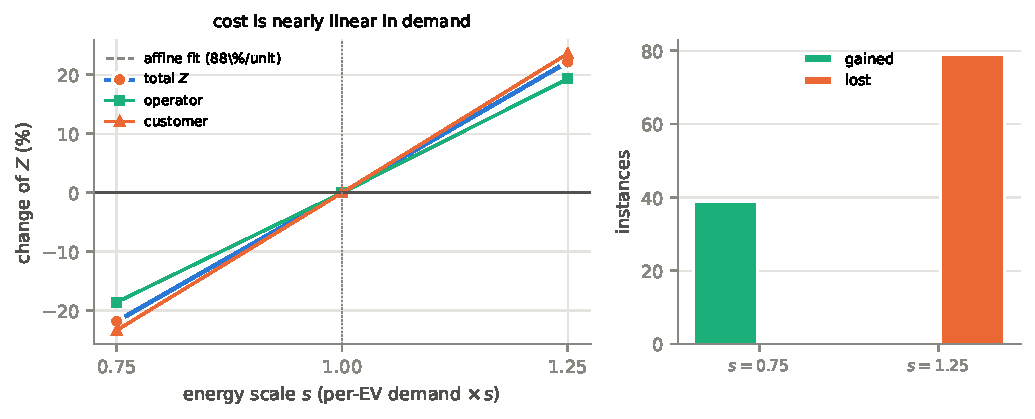
\includegraphics[width=\textwidth]{figures/exp_e10.pdf}
\caption{E10 charging demand. Left: change of $Z$ (and its operator/customer parts) against the energy scale $s$; the dashed line is the affine fit through the baseline. Right: instances that gain or lose a feasible plan.}
\label{fig:e10}
\end{figure}

\begin{table}[H]
\centering
\caption{E10, retrained RL. The baseline is $s=1$ (no change).}
\footnotesize
\begin{adjustbox}{max width=\linewidth}
\begin{tabular}{@{}llrrrrrr@{}}
\toprule
variant & what changes & \shortstack{$\Delta Z$\\\%} & \shortstack{$\Delta$\\oper. \%} & \shortstack{$\Delta$\\cust. \%} & gained & lost & paired \\
\midrule
E10\_demand\_0.75 & energy per EV x0.75 ($-$25 \%) & $-$21.82 & $-$18.59 & $-$23.35 & 39 & 0 & 500 \\
E10\_demand\_1.25 & energy per EV x1.25 ($+$25 \%) & $+$22.19 & $+$19.33 & $+$23.57 & 0 & 79 & 421 \\
\bottomrule
\end{tabular}
\end{adjustbox}

\end{table}

\subsection{What the numbers say}
\begin{itemize}
  \item \textbf{The response is large and nearly symmetric}: $-25$\,\% energy moves $Z$ by $-$\feTenDownDzAbs\,\%, $+25$\,\% moves it by \feTenUpDz\,\%. Operator cost and customer cost move together and in the same proportion.
  \item \textbf{It is nearly linear}: the three points ($s=0.75,1,1.25$) sit almost on a straight line through the baseline (Figure~\ref{fig:e10}, left), with a slope of about \feTenSlope\,\% per unit of~$s$.
  \item \textbf{Feasibility moves too}: $+25$\,\% energy strands \feTenUpLost{} instances (longer sessions miss the deadline), $-25$\,\% rescues \feTenDownGain.
\end{itemize}

\inshort{Charging demand is the single most powerful of the three analysis factors for the cost: a $\pm25$\,\% change in energy per car moves $Z$ by about $\pm22$\,\%, almost one-for-one.}

\subsection{Why: the cost is affine in demand}

\begin{keybox}
\textbf{Proposition 4 (energy affinity).} Scale every EV's energy demand by $s$: $E_i\!\to\! sE_i$. Then the total cost is affine in $s$,
\[
Z(s)=a+b\,s,
\]
where $b$ collects the terms proportional to the energies and $a$ the terms independent of them.\\[2pt]
\textbf{Proof.} Each objective term is one of two kinds. \emph{Energy-proportional} (each scales by $s$ when all $E_i$ do): the FCS charging time $\tau^F_i=60sE_i/P^F$ and the van charging time, so their time-costs; the operator's electricity $Z_4=\pi\sum_i sE_i$; the perceived tariff $Z_5=\sum_i \mu_i\,p\,sE_i$. \emph{Energy-independent}: van driving $Z_2$ (road distance), van dispatch $Z_3$ (a fixed cost per van used), and the drive-to-station time inside $Z_6$ (set by geometry, not by $E_i$). Summing a group that scales linearly with $s$ and a group that does not gives $Z(s)=bs+a$. $\square$
\end{keybox}

\begin{keybox}
\textbf{Corollary (elasticity and symmetry).} The elasticity of cost to demand at the baseline is
\[
\varepsilon=\left.\frac{dZ/Z}{ds/s}\right|_{s=1}=\frac{b}{a+b},
\qquad\text{so}\qquad
\frac{\Delta Z}{Z}(s)=\varepsilon\,(s-1).
\]
Hence the percentage change is a straight line through the baseline with slope $100\,\varepsilon$, and equal-and-opposite for $\pm\delta$. Measured slope $\approx\feTenSlope$ gives $\varepsilon\approx\feTenElastic$: about \feTenElastic{} of the cost scales directly with energy.\\[2pt]
\textbf{Proof.} From $Z(s)=a+bs$, $Z(1)=a+b$ and $\Delta Z/Z=(Z(s)-Z(1))/Z(1)=b(s-1)/(a+b)=\varepsilon(s-1)$; the slope in $s$ is $100\varepsilon$ and $\Delta Z/Z(1\pm\delta)=\pm\varepsilon\delta$ is symmetric. $\square$
\end{keybox}

The elasticity is below~1 because a share $a/(a+b)=1-\varepsilon\approx\feTenNonElastic\,\%$ of the cost does \emph{not} scale with energy. The baseline cost breakdown names this share almost exactly: van driving ($Z_2$, \fshareZTwo\,\%) and dispatch ($Z_3$, \fshareZThree\,\%) are purely geometric, and together with the fixed drive-to-station time they make up the roughly \feTenNonElastic\,\% that stays put while everything else --- the tariff ($Z_5$, \fshareZFive\,\%), the operator energy ($Z_4$, \fshareZFour\,\%) and the charging-time cost --- grows with $s$. The small departure from perfect symmetry ($-$\feTenDownDzAbs\,\% vs \feTenUpDz\,\%) is not a failure of the theory: it comes from the feasible set itself changing with $s$ (\feTenUpLost{} instances lost at $s=1.25$ against \feTenDownGain{} gained at $s=0.75$), so the two sides are averaged over slightly different instances.

\subsection{The three analysis factors side by side}

With E9 and E10 in hand, the three factors the course asks about can be ranked by their effect on the cost $Z$:
\begin{enumerate}
  \item \textbf{Charging demand (E10)}: $\pm25$\,\% energy $\Rightarrow$ about $\pm22$\,\% on $Z$ (elasticity \feTenElastic). The strongest lever, because most of $Z$ is energy-proportional.
  \item \textbf{Station power (E9)}: halving/doubling $\Rightarrow$ $+\feNinePowHalfDz$\,\% / $-$\feNinePowDblDzAbs\,\%, through the charging-time law $\tau^F\propto1/P^F$.
  \item \textbf{Mobile chargers (E2)}: the fleet \emph{size} barely touches the cost (about 0\,\% at the optima) and acts almost entirely on feasibility; cutting seats per van costs about $+1.3$\,\%.
  \item \textbf{Station guns (E9)}: $+\feNineGunsHalfDz$\,\% / $-$\feNineGunsDblDzAbs\,\%, the weakest cost lever, acting only through queueing.
\end{enumerate}
All three factors, however, share one role that the cost figures hide: at the hard end they decide \emph{feasibility}. Too little energy headroom, too few guns, too little power or too small a fleet each strand cars that cannot be charged before the deadline --- which is why every variant above also shows instances gained or lost.

\inshort{Because about \feTenElastic{} of $Z$ is proportional to the energy charged, the cost is essentially linear in demand and demand is the biggest single lever; station power is next (a convex $1/P$ law), the van fleet and the gun count move the cost little but govern feasibility.}
